\subsection[Konfiguracja urządzenia wykonującego (Michał Krakowiak)]{Konfiguracja urządzenia wykonującego}
W tym rodziale można całkiem sporo napisać o usb gadget configfs, nie ma takich rzeczy w programie studiów, a wykorzystaliśmy to do skonfigurowania rpi0 do działania jako klawiatura
Uzyskanie zamierzonego efektu wymaga odpowiedniego oprogramowania pożądanej funkcjonalności oraz wcześniejszego skonfigurowania urządzenia wykonującego. Wszystkie urządzenia wykonujące przynależące do realizowanego systemu działają pod kontrolą dedykowanej dystrybucji systemu operacyjnego Linux. Umożliwia do sprawdzenie problemu konfiguracji do skorzystania z istniejących interfejsów jądra systemu operacyjnego służących do tworzenia tzw. gadżetów USB. 
Termin gadżet USB używany jest do określenia urządzenia posiadającego własny kontroler urządzenia USB (ang. USB device controller, UDC) oraz możliwość podłączenia do hosta USB w celu udostępnienia mu pewnych dodatkowych funkcjonalności. Skonfigurowane w ten sposób urządzenie rozpoznawane jest przez hosta jako zbiór konfiguracji, z których każda zawiera interfejsy (nazywanych też funkcjami). System operacyjny linux dostarcza wielu gotowych funkcji urządzeń USB np. obsługę protokołu HID.
Realizowana konfiguracja korzysta z interfejsu USB Gadget Configfs, który pozwala na definiowanie konfiguracji i funkcjonalności złożonych gadżetów USB (czyli takich, które mogą udostępniać więcej niż jedną funkcjonalność) z poziomu przestrzeni adresowej użytkownika i nie wymaga realizacji własnych modułów jądra systemu operacyjnego.
Aktywacja interfejsu USB gadget configfs wymaga załadowania dodatkowego modułu jądra:
modprobe libcomposite
Proces kreowania nowego urządzenia polega na wykonaniu poszczególnych operacji na plikach w nowo zamontowanym katalogu
\begin{figure}[H]
    \centering
    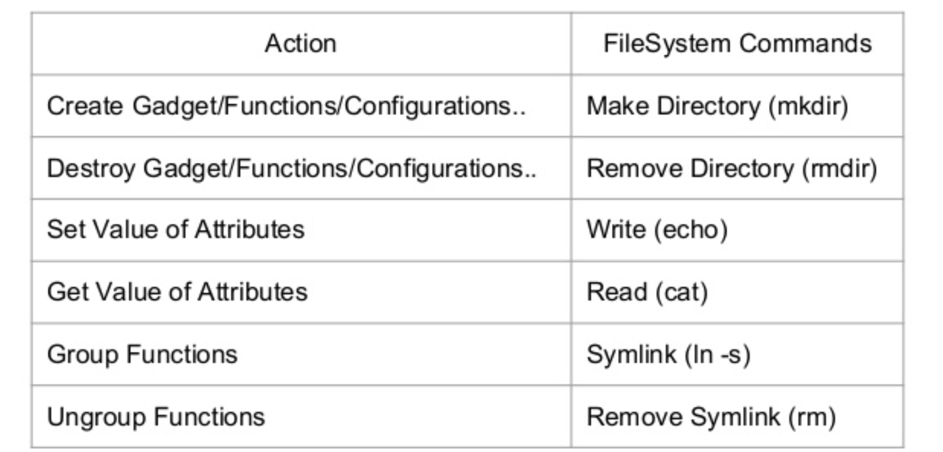
\includegraphics[width=\textwidth]{mk06}
    \caption{tabelka}
    \label{fig:tabelka}
\end{figure}
\begin{figure}[H]
    \centering
    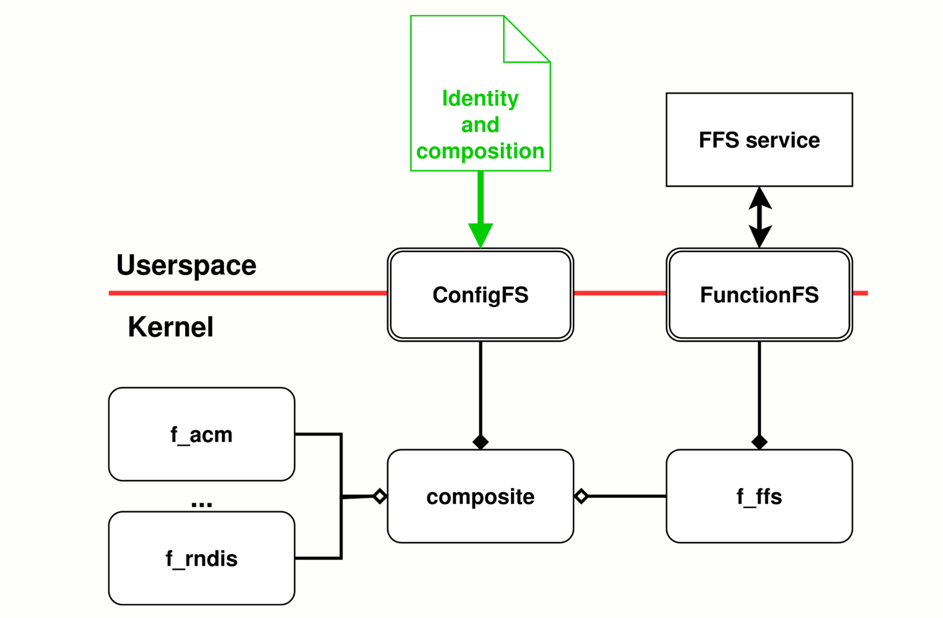
\includegraphics[width=\textwidth]{mk01}
    \caption{Configs}
    \label{fig:configfs}
\end{figure}
